	\subsection{Продолжение нормирований и ветвление}	


	Пусть тпеперь $L/K$~--- конечное расширение, $\v$~--- дискретное номрирование на $K$, а $w$~---- дискретное нормирование на $L$. 

	\begin{example}
		Пусть $L/\Q$~--- конечное расширение. Пусть $p$~--- простое число, тогда на $\Q$ у нас есть $p$-адическое нормирование $\v_{p}$. С другой стороны, 
		\[
			p\cO_{L} = \fp_{1}^{e_1} \cdot \ldots \fp_{k}^{e_k}
		\]
		и каждому простому соотвествует нормирование $w_{\fp_i}$. Легко видеть, что $w_{\fp_i}(x) = e_i \v_{p}(x)$. 
	\end{example}

	\begin{statement} 
		Следующие условия равносильны: 

		\begin{enumerate}
			\item Существует $e \in \N\colon \forall x \in K \ w(x) = e\v(x)$.

			\item $\cO_{\v} \subset \cO_{w}$.

			\item $\fm_{\v} \subset \fm_{w}$.

			\item $\fm_{\v} = \fm_{w} \cap \cO_{\v}$.
		\end{enumerate}
	\end{statement}
	\begin{proof}
		Во-первых, ясно, что их первого условия следуют все остальные. Покажем, что $\bf{2)} \implies \bf{1)}$. Нормирование $w$ на поле $L$ мы можем ограничить на поле $K$, т.е. рассмотреть $w\vert_{K}$. Вообще говоря, такое ограничение может и не быть нормированием, так как, ясно, что $\Im{w\vert_{K}}$ может не совпадать с $\Z$. В то же время, это некоторая подгруппа в $\Z$, предположим, что $\Im{w\vert_{K}} = e\Z$. Во-первых, $e \neq 0$. Действительно, так как $L$ алгебраично над $K$, любой $x \in L$ мы можем записать, как 
		\[
			x^n + a_{n - 1}x^{n - 1} + a_0 = 0 \implies x^n = -(a_{n - 1}x^{n - 1} + a_0), \quad a_j \in K.
		\]
		и взяв нормирование слева и справа мы получим противоречие. Действительно, если $w(x) \neq 0$, то 
		\[
			w(x^n) = nw(x) , \quad w(-a_j x^j) = w(a_j) + jw(x) = w(x),
		\]
		откуда мы получаем, что 
		\[
			nw(x) = \min(0, (n - 1)w(x)) \implies w(x) = 0
		\]
		и по произвольности $x \in L$ мы получаем, что $w = 0$, что даёт нам противоречие. 


		Тогда $e > 0$ и мы можем рассмотреть функцию $\v' = \frac{w\vert_{K}}{e}$, которая уже будет нормированием на $K$. Тогда мы получаем, что $\cO_{\v} \subset \cO_{\v'}$, а отсюда, по лемме~\ref{ant_2_lemma_1}, $\v = \v'$.  

		Равносильность остальных условий доказывается аналогично. 
	\end{proof}

	\begin{definition} 
		Если хотя бы одно из этих условий выполнено, то говорят, что $w \mid \v$ (или, что нормирование $w$ \emph{находится над} нормированием $\v$, или же, $w$ \emph{продолжает} $\v$). 
	\end{definition}

	Пусть $L/K$~--- конечное сепарабельное расширение, $\v$~--- нормирование на $K$, $\cO_{\v}$~--- кольцо нормирования. Напомним знакомое нам из коммутативной алгебры определение:

	\begin{definition} 
		Кольцо $A$ называется \emph{дедекиндовым}, если оно 
		\begin{itemize}
			\item нётерово

			\item целостное

			\item целозамкнутое 

			\item размерности 1.
		\end{itemize}
	\end{definition}

	В коммутативной алгебре у нас была такая теорема:

	\begin{theorem} 
		Пусть $A$~--- Дедекиндово кольцо, $K$~--- его поле частных, $L/K$~--- конечное расщирение (полей), а $B = \Int_{L}{A}$. Тогда $B$~--- дедекиндово. 
	\end{theorem}

	В нашей ситуации $A = \cO_{\v}$, а $B = \Int_{L}(A)$. Пусть  $\fm_{\v} = \fp$ и рассмотрим $\fp B$, он раскладывается в произведение простых: 

	\[
		\fp B = \prod_{i = 1}^{n} \fp_{i}^{e_i} 
	\]

	Каждая локализация $B_{\fp_i}$ является дискретно-нормированным кольцом (и, более того, кольцом нормирования $w_i$). Кроме того, все нормирования $w_i$, связанные с идеалами $\fp_i$, продолжают нормирование $\v$ (т.е. $w_i \mid \v$) и, это в точности все нормирования, продолжающие нормирование $\v$.

	В самом деле, если $w$ продолжает $\v$, то $(w \vert v \implies \fm_v \subset \fm_{w} \implies \fm_{v}B \divby \fm_{w})$  $\fm_{w} \cap B$~--- простой идеал, висящий над идеалом $\fp$, то есть, один из $\fp_i$. Пусть $\fm_{w} \cap B = \fp_i$, тогда $\fm_{w} \cap B_{\fp_i} = \fp_i B_{\fp_i}$. Тогда $\fm_{w} \cap \cO_{w_i} = \fm_{w} \cap B_{\fp_i} = \fm_{w_i}$, откуда $w = w_i$.

	Как мы уже отмечали, $B_{\fp_i} /\fp_i B_{\fp_i} = \cO_{w_i}/\fm_{w_i}$. Положим 
	\[
		f_i = [\cO_{w_i}/\fm_{w_i} : A/\fp] = [\Bbbk_{w_i} : \Bbbk_{\v}] 
	\]
	и будем (как и в первой части курса) называть $f_i$ \bf{степенью инерции}.

	Отметим так же, что, как и в случае колец целых, $B$~--- свободный $\cO_{\v}$-модуль ранга $n$ (как и кольцо целых $\cO_{K}$, которое было свободным $\Z$-модулем ранга $n$).


	\begin{theorem} 
		Для индексов ветвления и степеней инерции справедлива следующая формула: 
		\[
			\sum_{i = 1}^{k} e_i f_i = n.
		\]
	\end{theorem}
	\begin{proof}
		Пусть $\fp = \fm_{\v}$. Так как $B$~--- свободный $\cO_{\v}$-модуль ранга $n$, ясно, что что $B/\fp B$~--- векторное пространство над $A/\fp$ размерности $n$. 
		\[
			B/\fp B \cong B/\prod \fp_i^{e_i} = B/\fp_{i}^{e_1} \times  B/\fp_{i}^{e_2} \times \ldots \times  B/\fp_{k}^{e_k}.
		\]
		Вычисляя размерности обеих частей равенства и приравнивая, мы получаем 
		\[
			n = \sum_{i = 1}^{k} \dim_{A/\fm} B/\fp_i^{e_i}.
		\]
		Рассмотрим на кольце $B$ фильтрацию степенями идеалов $\fp_i$:
		\[
			\fp_{i}^{e_i} \subset \fp_i^{e_i - 1} \subset \ldots \subset \fp_i \subset B.
		\]
		Посмотрим на факторы этой фильтрации, то есть, на  $\fp_{i}^{m}/\fp_{i}^{m + 1}$, они являются векторными пространствами над $A/\fp$. Покажем, что $\forall m \ge 1$ $B/\fp_i \cong \fp_i^m / \fp_i^{m + 1}$. Выберем $x \in \fp_i^{m}\setminus \fp_{i}^{m + 1}$ и отображение $m_{x}\colon B/\fp_i \to \fp_i^m/\fp_i^{m + 1}, \ y \mapsto xy$. Вполне ясно, что это корректно определённый гомоморфизм, вычислим его ядро.  Рассмотрим $y \in B$ такой, что $xy \in \fp_i^{m + 1}$ и покажем, что тогда $y \in \fp_i$. Рассмотрим главный идеал $(xy)$. Так как $xy \in \fp_i^{m + 1}$, его разложение на простые имеет вид 
		\[
			(xy) = \fp_i^{m + 1} \cdot I.
		\]
		С другой стороны, $(x) = \fp_i^{m} \cdot J, \ J \notdivby \fp_i$ и тогда  $(y) = \fp_i \cdot \widetilde{J}$, откуда $y \in \fp_i$. Значит, мы показали, что $\ker{m_{x}} = \{ 0\}$. Сюръективность отображения $m_{x}$ следует из того, что $(x) + \fp_{i}^{m + 1} = \fp_{i}^m$. Так как $x \in \fp_i^m$, очевидно, что левая часть лежит в правой. Тогда $(x) + \fp_{i}^{m + 1} =  \fp_i^m \cdot I$, покажем, что $I = (1)$. Предположим противное, тогда 
		\[
			I = \fp_i^{s} \cdot \fq_{1}^{r_1} \cdot \ldots \fq_{\ell}^{r_{\ell}}, \quad \fq_j \neq \fp_i.
		\]

		Тогда $I = \fp_{i}^{s}$, откуда $(x) + \fp_{i}^{m + 1} = \fp_{i}^{m + s}$. Предположим, что $s$ положительно. Тогда $(x) \subset \fp_i^{m + 1}$, что противоречит тому, что мы брали $x \in \fp_i^{m}\setminus \fp_{i}^{m + 1}$. Тогда мы показали, что 
		\[
			B/\fp_i \cong \fp_i^m/\fp_i^{m + 1},
		\]
		и отсюда уже следует теорема: 
		\begin{multline*}
			B/\fp_{i}^{e_i} \cong \frac{B}{\fp_{i}} \cdot \frac{\fp_i}{\fp_{i}^2}  \cdot \ldots \frac{\fp_i^{e_i - 1}}{\fp_{i}^{e_i}} \implies \\ \implies \dim_{A/\fp} B/\fp_i^{e_i} = \dim_{A/\fp}{B/\fp_i} + \dim_{A/\fp}{\fp_i/\fp_i^2} + \ldots + \dim_{A/\fp}{\fp_i^{e_i - 1}/\fp_i^{e_i}} = e_i \cdot \dim_{A/\fp}{B/\fp_i} = e_i \cdot f_i.  
		\end{multline*}
	\end{proof}

	Теперь посмотрим, что будет происходить в \bf{несепарабельном} случае. 

	В этом случае наше расширение раскладывается в башню 
	\begin{center}
		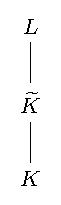
\includegraphics{lectures/6/pictures/cd_22.pdf}
	\end{center}

	
 	
 	где расширение $L/\widetilde{K}$ чисто несепарабельно. Если $\Char{K} = 0$, то $\widetilde{K} = L$. Если же $\Char{K} = p$,то чисто несепарабельное расширение, в свою очередь, раскладывается в башню \emph{элементарных} чисто несепарабельных расширений:
 	\[
 		\widetilde{K} \subset K_1 \subset K_2 \subset \ldots \subset K_m \subset L.
 	\]
 	Каждое из них устроено следующим образом: $K_{i + 1} = K_i\lr*{\sqrt[p]{a}}$, где $a \in K_i$ и $a$ не является $p$-й степенью, а $p = \Char{K}$.  

 	Докажем, что каждое нормирование на $K_i$ мы можем продолжить на $K_{i + 1}$. 

 	\begin{lemma} 
 		Пусть $F \subset F_1 \subset F_2$, причем на этих полях есть нормирования $\v, \v_1$ и $\v_2$ соответственно. Тогда
 		\[
 			\begin{cases} \v_1 \text{ продолжает } \v \\ \v_2 \text{ продолжает } \v_1 \end{cases} \implies \v_2 \text{ продолжает } \v.
 		\]
 	\end{lemma}
 	\begin{proof}
 		В самом деле, нам известно, что 
 		\[
 			\forall x \in F \ \v_1(x) = e_1 \v(x), \quad \forall y \in F_1 \ \v_2(y) = e_2 \v_1(y).
 		\]
 		Тогда мы получаем, что $\forall x \in F \ \v_2(x) = e_2 \v_1(x) = e_2 e_1 \v(x)$, что даёт нам, что $\v_2$ продолжает $\v$.
 	\end{proof}

 	\begin{lemma} 
 		Пусть $L/F$~--- элементарное чисто несепарабельное расширение, то есть $L = F\lr*{\sqrt[p]{a}}$, а $\v$~--- нормирование на $F$. Тогда у нормирования $\v$ существует единственное продолжение на $L$.
 	\end{lemma}
 	\begin{proof}
 		 Сначала отметим, что возводя элемент поля $L$ в степень $p$, мы неизбежно получим элемент поля $F$, так как любой элемент $L$ мы можем записать как
 		 \[
 		 	x = f_0 + f_1 \sqrt[p]{a} + \ldots + f_{p - 1} \sqrt[p]{a^{p - 1}}.
 		 \]



 		Рассмотрим функцию $\varphi\colon L \to \Z$, $\varphi(x) = \v\lr*{x^p}$. Ясно, что $\varphi$ является гомоморфизмом $L^* \to \Z$. Кроме того, 
 		\[
 			\varphi(x + y) = \v\lr*{(x + y)^p} = \v\lr*{x^p + y^p} \ge \min\lr*{\v\lr*{x^p}, \v\lr*{y^p}} = \min\lr*{\varphi(x), \varphi(y)}. 
 		\]
 		Опять же, тогда $\Im{\varphi} = f\Z$, где $f \in \N$. Нетрудно заметить, что так как для $x \in F \ \varphi(x) = p\v(x)$, откуда $p \in \Im{\varphi}$, то есть, $f = 1$ или $f = p$. Мы можем рассмотреть нормирование 
 		\[
 			w = \frac{\varphi}{f}, \quad x \in F \rightsquigarrow w(x) = \frac{\v\lr*{x^p}}{f} = \frac{p}{f}\v(x) \rightsquigarrow w \mid \v.
 		\]	

 		Теперь докажем единственность. Пусть $w'$ продолжает нормирование $\v$ с индексом ветвления $e$. Возьмём $x \in L$, тогда 
 		\[
			w'\lr*{x^p} = e \v\lr*{x^p} = ef w(x),
		\]	
		а с другой стороны, $w'(x) = p w'(x)$, откуда $w'(x) = \frac{ef}{p}w(x)$. Подставляя в это равенство локальный параметр для нормирования $w$, мы получаем, что $\frac{ef}{p} = 1$, откуда $w = w'$. 
 	\end{proof}

 	\begin{lemma} 
 		Пусть $L/F$~--- чисто несепарабельное расширение, а $\v$~--- нормирование на $F$. Тогда у нормирования $\v$ существует единственное продолжение на $L$.
 	\end{lemma}
 	\begin{proof}
 		Разложим наше чисто несепарабельное расширение в башню элементарных чисто несепарабельных: 
 		\[
 			F_0 \subset F_1 \subset F_2 \subset \ldots \subset F_n = L.
 		\]

 		Тогда, по предыдущей лемме у нас есть последователньость нормирований $\v, w_1, \ldots, w_n$, каждое из которых продолжает другое. Соответственно, так мы получаем существование. Теперь проверим единственность. 

 		Пусть $w$~--- нормирование на $L$, продолжающее $v$. Докажем, что оно продолжает $w_{n - 1}$ (и, отсюда будет следовать, что оно совпадает с $w_{n}$). Пусть $w(x) = e\v(x) \ \forall x \in F$. Заметим теперь, что

 		\[
 			F_n^{p} \subset F_{n - 1}, \ F_{n - 1}^{p} \subset F_{n - 2}, \ \ldots, F_1^p \subset F_0 \implies F_{n - 1}^{p^{n - 1}} \subset F.
 		\]

 		Тогда мы имеем 
 		\[ 
 		\forall x \in F_{n - 1} \ w\lr*{x^{p^{n - 1}}} = e\v\lr*{x^{p^{n - 1}}} = \frac{e w_{n - 1}\lr*{x^{p^{n - 1}}}}{e'} = \frac{e p^{n - 1}}{e'} w_{n - 1}(x).
 		\]
 		С другой же стороны, $p^{n - 1}w(x) = \frac{e}{e'} p^{n - 1}w_{n - 1}(x) \ \forall x \in F_{n - 1}$. Подставляя в это равенство локальный параметр для нормирования $w_{n - 1}$ мы получаем, что $e/e' \in \Z$, откуда $w \mid w_{n - 1}$, а значит, $w = w_{n}$.
 	\end{proof}

 	Пусть теперь $K$~--- полное поле относительно нормирования $\v$, а $L/K$~--- конечное расширение. Докажем вот такую теорему: 

 	\begin{theorem} 
 		В случае полного относительно нормирования $\v$ поля $K$ существует единственное продолжение $\v$ на $L$. Поле $L$ является полным относительно этого нормирования. 
 	\end{theorem}
 	\begin{proof}

 	Рассмотрим $L$, как векторное пространство над $K$, пусть $V \subset L$~--- ненулевое подпространство. Мы знаем, что какое-то продолжение нормирования $\v$ на $L$ существует, обозначим его за $w$. Рассмотрим последовательность  $\{ x_i \}, \ x_i \in V$ и обозначим за $\{ v_j \}$  базис $V$. Разложим $x_i$ по базису: 
 	\[
 		x_i = \sum_{j} a_{i j} v_{j}, \quad a_{i j} \in K.
 	\]

 	\begin{lemma} 
 		Если $x_i \xrightarrow{|\cdot|_{w}} 0$, то $a_{i j} \xrightarrow{|\cdot|_{\v}} 0$ для всех $j$. 
 	\end{lemma}
 	\begin{proof}
 		Будем вести доказательство индукцией по размерности $V$. В случае, когда она равна единице, утверждение тривиально. Не умаляя общности, пусть $j = 1$. Предположим, что $a_{i 1} \not\xrightarrow{|\cdot|_{\v}} 0$. Тогда, переходя к подпоследовательности, мы можем полагать, что $\exists c > 0 \ \colon \forall i \ |a_{i 1}|_{\v} > c$.

 		Рассмотрим 
 		\[ 
 			\widetilde{x_i} = \frac{x_i}{a_{i 1}} = v_1 + y_{2i} v_2 + \ldots + y_{mi} v_m,  
 		\] 
 		где $m = \dim{V}$. 


 		Ясно, что $\widetilde{x_i} \xrightarrow{|\cdot|_{w}} 0$. Заметим, что $t_i = \widetilde{x_{i + 1}} - x_{i} \in \Span\lr*{v_2, \ldots, v_{m},}$, а тогда по предположению индукции 
 		\[ 
 			y_{j,i+ 1} - y_{j, i} \xrightarrow{|\cdot|_{\v}} 0 \quad \forall j.
 		\]	
 		 Тогда $\{ y_{j, i} \}_{i \in \N}$~--- последовательность Коши и, так как поле полное, она имеет предел. Пусть 
 		\[
 			\lim_{i \to \infty} \{ y_{j, i} \}_{i \in \N} = s_{j}
 		\]

 		\[
 			0 \xleftarrow{i \to \infty} \widetilde{x_i} = \frac{x_i}{a_{i 1}} = v_1 + y_{2i} v_2 + \ldots + y_{mi} v_m \xrightarrow{i \to \infty} v_1 + s_2 v_2 + \ldots + s_m v_m.
 		\]
 		что противоречит тому, что $\{ v_i \}$~--- базис. 

 	\end{proof}

 	Продолжим доказательство теоремы. Если $\{ x_i \}$~--- последовательность Коши, то по лемме $\{ a_{i j} \}$~--- тоже последовательность Коши. Тогда, так как пле полное, $a_{i j} \xrightarrow{i \to \infty} s_j$, откуда 
 	\[
 		x_i = \sum_{j} a_{i j} v_{j} \xrightarrow{|\cdot|_{w}} \sum_{j} s_j v_j,
 	\]
 	то есть поле будет полным относительно нормирования $w$. 

 	Теперь докажем единственность. Пусть $w' \neq w$~--- другое продолжение нормирования $\v$. Тогда по аппроксимационной теореме мы можем найти $x_i \in L$ такие, что 
 	\[
 		x_i \xrightarrow{|\cdot|_w} 0, \quad x_i \not\xrightarrow{|\cdot|_{w'}} 0.
 	\]
 	Но из первого условия по лемме мы имеем $a_{i j} \xrightarrow{|\cdot|_{v}}$, а отсюда следует, что $x_i \xrightarrow{|\cdot|_{w'}} 0$, что противоречит предположению выше. 


 	\end{proof} 

 	Таким образом мы доказали еще и такую теорему:

 	\begin{theorem} 
 		Пусть $L/K$~--- конечное расширение, $\v$~--- нормирование на $K$. Тогда $\v$ можно продолжить на $L$.
 	\end{theorem}

 	\begin{proof}
 		
 	\end{proof}

 	\begin{homework}
 		 Задачи: 

 		 \begin{enumerate}
 		 	\item  Докажите лемму Гензеля для полных полей:
 		 	\begin{theorem}[Лемма Гензеля для полных полей] 
 		Пусть $(K, \v)$~--- полное поле относительно нормирования $\v$, $\cO = \cO_{\v}, \ \fm = \fm_{\v}$. Пусть $f \in \cO[x]$ и $f \neq 0 \pmod{\fm}$. Предположим, что 
 		\[
 			\overline{f_1} = \overline{g_1} \overline{h_1}, \quad (\overline{g_1}, \overline{h_1}) = (1) \text{ над } \Bbbk = \cO/\fm.
 		\]

 		Тогда $\exists g, h \in \cO[x]\colon $
 		\vspace{-2mm}
 		\begin{enumerate}
 			\item $f = gh$.
 			\item $\deg{g} = \deg{\overline{g_1}}$.
 			\item $\overline{g} = \overline{g_1}, \ \overline{h} = \overline{h_1}$.
 		\end{enumerate}
 	\end{theorem}

 	\item Докажите следствие из леммы Гензеля: 

 	\begin{corollary}[Из леммы Гензеля]
 		Пусть $f \in K[x]$~--- унитарный неприводимый многочлен над полным полем $K$, $f(0) \in \cO_{\v}$. Тогда $f \in \cO_{v}[x]$. 

	\item Пусть $L/K$~--- конечное расширение, а поле $K$~--- полное относительно нормирования $\v$. Положим $\varphi(x) = \v(\Nm_{L/K}(x))$. Тогда: 

		\begin{enumerate}
			\item $\varphi\colon L^* \to \Z$~--- гомоморфизм. 

			\item $\varphi(x + y) \ge \min(\varphi(x), \varphi(y))$.

			\item $\frac{\varphi}{f}$~--- нормирование на $L$, продолжающее $\v$. 

			\item Пусть $(K, \v)$~--- произвольное нормированное поле, а $f$~--- мноочлен Эйзенштейна, то есть 
			\[
				f(x) = x^n + a_{n - 1} x^{n - 1} + \ldots + a_0, \quad \v(a_i) > 0, \ \v(a_0) = 1.	
			\] 
			Тогда 
			\begin{enumerate}
				\item $f$ неприводим. 
				\item Нормирование $\v$ однозначно продолжается на поле $L = K[x]/(f)$, причём $e = n, \ f = 1$. 
			\end{enumerate}
		\end{enumerate}
 	\end{corollary}
 		 \end{enumerate}
 	\end{homework}

 	
 	

 	


